\begin{appendix}
\chapter{Anhang}
\label{chap:anhang}

\section{Flächenflugzeug}
Der in Gleichung \ref{eq:geschw_flaechenflugzeug} aufgeführte Zusammenhang entsteht aus dem Verhältnis der Fluggeschwindigkeiten bei konstanten Auftriebsbeiwert. Aus der Definition des Auftriebsbeiwertes
\begin{equation}
	c_{A} = \frac{A}{\rho/2\cdot V^2\cdot S}
\end{equation}
entsteht durch Umformen die Beziehung für die Geschwindigkeit
\begin{equation}
	V = \sqrt{\frac{2\cdot A}{\rho\cdot S \cdot c_{A}}} \eqend{.}
\end{equation}
Im Horizontalflug (\ensuremath{\gamma = 0}) kompensiert der Auftrieb lediglich die Gewichtskraft (Vgl. Gleichung \ref{eq:auftriebsgleichung_vereinfacht})
\begin{equation}
	A = G \eqend{.}
\end{equation}
Für jegliche Art von Steigflug (\ensuremath{\gamma \neq 0}) ist dies nicht mehr der Fall. Unter der Voraussetzung einer gleichen Gewichtskraft \ensuremath{m\cdot g}, gleicher Flügelfläche \ensuremath{S} und einem konstanten Auftriebsbeiwerts \ensuremath{c_{A}} ergibt sich für das Verhältnis der Geschwindigkeiten \ensuremath{V/V^\star}
\begin{equation}
	\frac{V}{V^\star} = \frac{\sqrt{\frac{2\cdot m \cdot g\cdot \cos\gamma}{\rho\cdot S \cdot c_{A}}}}{\sqrt{\frac{2\cdot m\cdot g}{\rho^\star \cdot S \cdot c_{A}}}} = \sqrt{\cos\gamma\cdot\frac{\rho^\star}{\rho}} \eqend{.}
\end{equation}\\

\section{Vergleich von normierter zur originalen Batteriezelle}
Für den Vergleich der Norm- mit der Originalzelle wird das Integral unterhalb der beiden Entladekurven für eine bestimmte Entladerate gebildet. Anschließend werden beide Flächen zu einander in Beziehung gesetzt 
\begin{equation}
	\text{Toleranz} = \frac{\text{F}_{Orig.}-\text{F}_{Norm}}{\text{F}_{Norm}} \eqend{.}
\end{equation} 
Im Sinne einer Genauigkeitssteigerung werden alle die Batterien in der Normzellenberechnung nicht berücksichtigt, deren individuelle Abweichung eine große Diskrepanz zur Standardabweichung aufweist. Der Vergleich zeigt, dass es starke Abweichungen der Batterie gibt. Die durchschnittliche Abweichung liegt für Entladeraten bis \SI{45}{1/h} deutlich über Null und steigt mit der Entladerate von \SI{8}{\%} auf \SI{17}{\%} bei \SI{45}{1/h}. Die Spannung der Normzelle ist somit im Durchschnitt kleiner als die der originalen Batteriezelle. Ab der Entladerate von \SI{50}{1/h} fällt die Abweichung drastisch auf \SI{-18}{\%} ab. 
\missingfigure{Abweichungsbilder}



\section{Steiggeschwindigkeit}
\begin{center}
\begin{figure}[H]
\begin{struktogramm}(163,160)
\while[5]{Für alle Bahngeschwindigkeiten}
	\assign[2]{Berechne Gesamtmasse}
	\assign[2]{Flugzeit für Höhenschritt berechnen}			
	\while[5]{Solange Abbruchkriterium nicht erreicht}
		\assign{Aerodynamik berechnen}
	\whileend
	\assign[2]{Schub berechnen}
	\assign[2]{Schub auf Propeller verteilen}
	\ifthenelse[10]{1}{4}{Schub zu gro\ss{}?}{ja}{nein}
		\assign[2]{Ergebnis verwerfen (NaN)}
		\change
		\assign[2]{Drehzahl und Drehmoment aus Propellerkennfeld interpolieren}
		\assign[2]{Motorzustand berechnen}
		\assign[2]{Zustand der Motorregler berechnen}
		\assign[2]{Zustand der Batterie neu berechnen}
		\assign[2]{Gesamtwirkungsgrad berechnen}
	\ifend
	\ifthenelse[10]{1}{1}{Werden Grenzen überschritten?}{ja}{nein}
		\assign[2]{Ergebnis verwerfen (NaN)}
		\change
		\assign[2]{Ergebnis beibehalten}
	\ifend
	\assign[2]{Speichern der aufgebrachten Energiemenge}
\whileend
\ifthenelse[10]{5}{1}{Sind die Werte NaN?}{nein}{ja}
	\while[5]{Solange Abbruchkriterium nicht erreicht}		
		\assign[2]{Finde den Index mit der geringsten verbrauchten Energiemenge}
		\ifthenelse[10]{1}{3}{Werte innerhalb Leistungsgrenzen?}{ja}{nein}
			\assign[2]{Verlasse Schleife}
			\change
			\assign[2]{Suche nächst kleinere Energiemenge}
		\ifend
	\whileend
	\assign[2]{Übergabe aller Leistungsparameter mit diesem Index}
		\change
	\assign[2]{Verwerfe alle Ergebnisse}
\ifend
\end{struktogramm}
\caption{Programmstruktur zur Ermittlung der optimalen Steiggeschwindigkeit}
\label{abb:steiggeschw}
\end{figure}
\end{center}

\section{Batteriemasse}
\begin{figure}[H]
\centering
	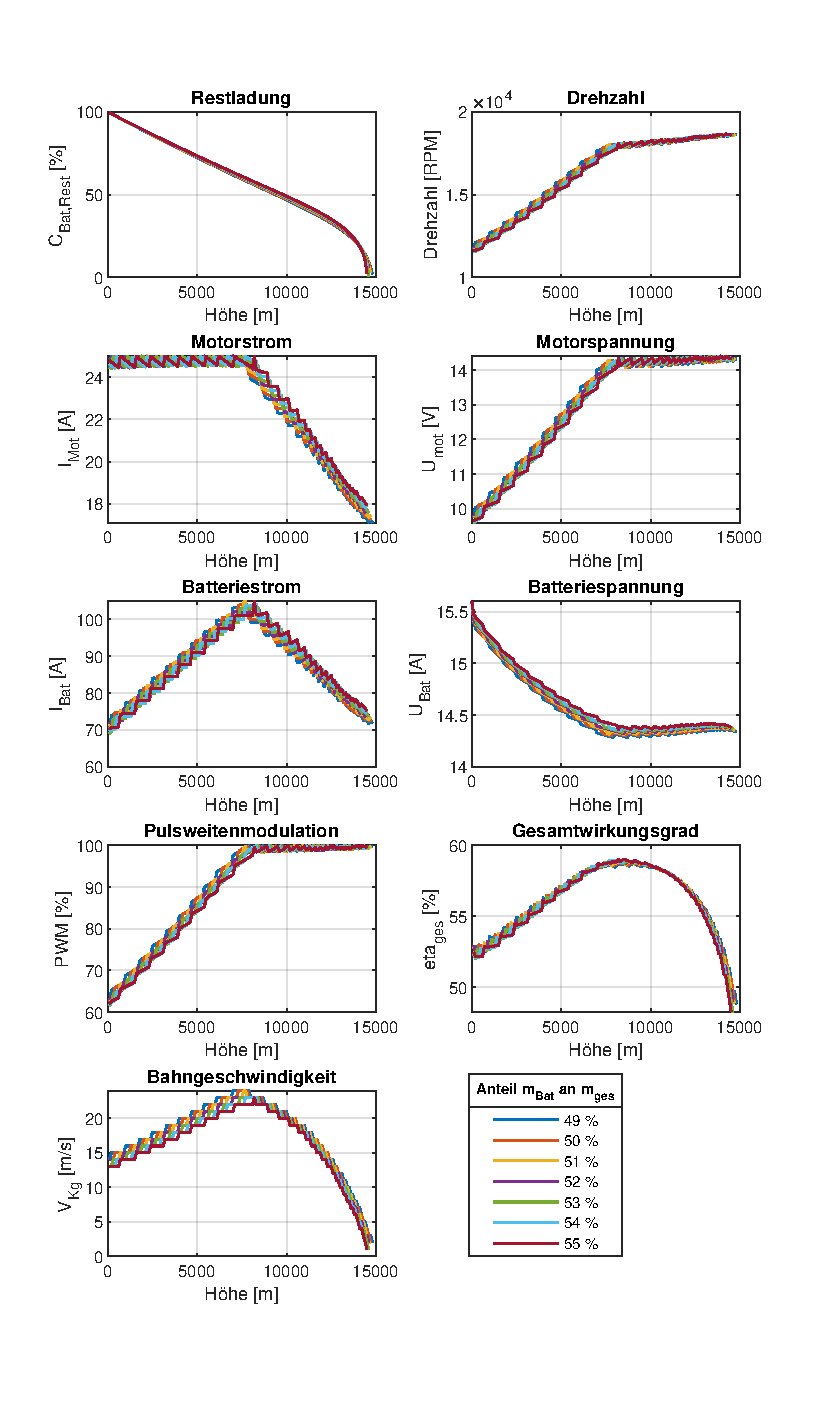
\includegraphics[scale=0.85]{Diagramme/Batteriemasse_genauer.pdf}
	\caption{genauere Untersuchung der Batteriemassenabhängigkeit (\ensuremath{m_{Mot}=\SI{106}{g}}, \ensuremath{K_V=\SI{1390}{RPM/V}}, \ensuremath{n_{Prop}=4}, \ensuremath{Propeller=\SI{10x3}{}}, \ensuremath{n_{Bat,cell}=4}, \ensuremath{u_{Wg}=\SI{10}{m/s}})}
	\label{abb:batteriemasse_genauer}
\end{figure}

\section{Verstellpropeller}

\begin{center}
\begin{figure}[H]
\begin{struktogramm}(163,160)
\assign[1]{Multicopter- und Umgebungsparameter festlegen (im Startskript)}
\assign[1]{Diskretisierungen (Geschwindigkeit, Höhe) festlegen}
\assign[1]{Aufruf des Hauptskripts: Leistungsberechnung starten}
\while[5]{Für alle Zeilen der APC-Datenbank}
	\ifthenelse[10]{1}{1}{Stimmt Durchmesser mit dem gesuchten überein?}{ja}{nein}
		\assign[2]{Gehe zur nächsten Zeile}
		\change
		\assign[2]{Lösche Zeile}
	\ifend
\whileend
\while[5]{Für alle Propeller}
	\assign[2]{Extrahiere Propellerkennfeld}
	\assign[2]{Speicher das Ergebnis unter fortlaufenden Nummern}
	\assign[2]{Erhöhe Propellerzähler}
\whileend
\assign[1]{Initialisierung der Parameterberechnung}
\while[5]{F\"ur alle Höhenabschnitte}
	\assign[1]{H\"ohe, Dichte, Luftdruck Temperatur berechnen}
	\assign[1]{arithmetische Mittelwert berechnen}
	\assign[1]{Schub- und Leistungskennfeld anpassen}
	\assign[2]{Initialisierung der Leistungsberechnung}
	\while[5]{Für alle Bahngeschwindigkeiten}
		\assign[2]{Initialisierungen}
		\while[5]{Für alle Propeller}
			\assign[2]{\texttt{\textbf{Leistungsberechnung}}}
			\assign[2]{Berechnung benötigter Energiemenge bei dieser Bahngeschwindigkeit mit diesem Propeller}
		\whileend
		\ifthenelse[10]{4}{1}{Sind die Werte NaN?}{nein}{ja}
			\while[5]{Solange Abbruchkriterium nicht erreicht}		
				\assign[2]{Finde den Index mit der geringsten verbrauchten Energiemenge}
				\ifthenelse[10]{1}{1}{Werte innerhalb Leistungsgrenzen?}{ja}{nein}
				\assign[2]{Verlasse Schleife}
				\change
				\assign[2]{Suche nächst kleinere Energiemenge}
				\ifend
			\whileend
			\assign[2]{Übergabe aller Leistungsparameter mit diesem Index}
			\change
			\assign[2]{Verwerfe alle Ergebnisse}
		\ifend
		\assign[2]{Berechne benötigte Energie für Steiggeschwindigkeit}
	\whileend
	\ifthenelse[10]{4}{1}{Sind die Werte NaN?}{nein}{ja}
		\while[5]{Solange Abbruchkriterium nicht erreicht}		
			\assign[2]{Finde den Index mit der geringsten verbrauchten Energiemenge}
			\ifthenelse[10]{1}{1}{Werte innerhalb Leistungsgrenzen?}{ja}{nein}
			\assign[2]{Verlasse Schleife}
			\change
			\assign[2]{Suche nächst kleinere Energiemenge}
			\ifend
		\whileend
		\assign[2]{Übergabe aller Leistungsparameter mit diesem Index}
		\change
		\assign[2]{Verwerfe alle Ergebnisse}
	\ifend
	\assign[2]{Erhöhe Zählervariable}
\whileend
\assign[2]{Ergebnisse der Leistungsparameter in Diagrammen speichern}
\assign[2]{Speichern der Diagramme in .pdf-Datei}
\end{struktogramm}
\caption{Programmstruktur die Untersuchung des Nutzens eines Verstellpropellers}
\label{abb:vpp}
\end{figure}
\end{center}


\section{Getriebe}

\begin{center}
\begin{figure}[H]
\begin{struktogramm}(163,210)
\assign[1]{Multicopter- und Umgebungsparameter festlegen (im Startskript)}
\assign[1]{Diskretisierungen (Getriebe, Geschwindigkeit, Höhe) festlegen}
\assign[1]{Aufruf des Hauptskripts: Leistungsberechnung starten}
\assign[1]{Initialisierung der Parameterberechnung}
\while[5]{F\"ur alle Höhenabschnitte}
	\assign[1]{H\"ohe, Dichte, Luftdruck Temperatur berechnen}
	\assign[1]{arithmetische Mittelwert berechnen}
	\assign[1]{Schub- und Leistungskennfeld anpassen}
	\assign[2]{Initialisierung der Leistungsberechnung}
	\while[5]{Für alle Bahngeschwindigkeiten}
		\assign[2]{Initialisierungen}
		\while[5]{Für alle Übersetzungen}
			\assign[2]{\textbf{Leistungsberechnung}}
		\whileend
		\ifthenelse[10]{4}{1}{Sind die Werte NaN?}{nein}{ja}
			\while[5]{Solange Abbruchkriterium nicht erreicht}		
				\assign[2]{Finde den Index mit der geringsten verbrauchten Energiemenge}
				\ifthenelse[10]{1}{1}{Werte innerhalb Leistungsgrenzen?}{ja}{nein}
				\assign[2]{Verlasse Schleife}
				\change
				\assign[2]{Suche nächst kleineren Energiemenge}
				\ifend
			\whileend
			\assign[2]{Übergabe aller Leistungsparameter mit diesem Index}
			\change
			\assign[2]{Verwerfe alle Ergebnisse}
		\ifend
		\assign[2]{Berechne benötigte Energie für Steiggeschwindigkeit}
	\whileend
	\ifthenelse[10]{4}{1}{Sind die Werte NaN?}{nein}{ja}
		\while[5]{Solange Abbruchkriterium nicht erreicht}		
			\assign[2]{Finde den Index mit der geringsten verbrauchten Energiemenge}
			\ifthenelse[10]{1}{1}{Werte innerhalb Leistungsgrenzen?}{ja}{nein}
			\assign[2]{Verlasse Schleife}
			\change
			\assign[2]{Suche nächst kleinere Energiemenge}
			\ifend
		\whileend
		\assign[2]{Übergabe aller Leistungsparameter mit diesem Index}
		\change
		\assign[2]{Verwerfe alle Ergebnisse}
	\ifend
	\assign[2]{Erhöhe Zählervariable}
\whileend
\assign[2]{Ergebnisse der Leistungsparameter in Diagrammen speichern}
\assign[2]{Speichern der Diagramme in .pdf-Datei}
\end{struktogramm}
\caption{Programmstruktur die Untersuchung des Nutzens eines Getriebes}
\label{abb:getriebe}
\end{figure}
\end{center}



\end{appendix}
